\section{Selective Symbolic Execution}

Symbolic execution~\cite{symbolic} is used to reason path-flow behavior of a program by tracing path constraint information collected during symbolic execution. This technique is useful in automated software testing such as increasing path coverage.

There exist two issues with regards to limited scalability of symbolic execution. The first issue is that this technique can be applied on only small program with at most thousands of lines of code. Note that symbolic execution collects states and constraints to keep track of path information in a program. During symbolic execution, the size of such states and constraints is exponential to the number of conditions (e.g., as if-else statements in program) in a program. This problem is called as path explosion. Due to such an exponential growth, the technique is not yet applied to large programs (e.g., program with more than millions lines of code).

The second issue is related to symbolic execution interacting with environments such as library or third-party program. Many programs are often interacting with environments such as external libraries to control network devices. For example, if a program under test uses external libraries, the program may require symbolic execution on external libraries as well. Such symbolic execution of environments could result in path explosion.

Ideally, testers often try to achieve covering all or specific paths of a system. However, in practice, covering such paths is not trivial due to limited scalability caused by path explosion. To address the issue, Chipounov et al.~\cite{selective} propose selective symbolic execution technique. The main idea of this technique, called selective symbolic execution (S$^2$E), combines both symbolic execution and concrete execution. More specifically, users specify portions (in a system) of interest. For example, portions of interest could be program related to CPU or memory usage to detect deadlock or memory leakage. S$^2$E explores such portions (of interest) symbolically (i.e., in-scope executions) and the remaining portions (of non-interest) concretely (i.e., out-scope executions). Therefore, execution of a program under test is back and forth between the symbolic and concrete executions based on which portions are executed.

S$^2$E can be practical since the authors observe that developers often focus on only small portion of code in a system (e.g., kernel module or newly added feature) instead of testing a whole system. S2E can be useful for many important software development tasks as follows.

\begin{figure}
\centering
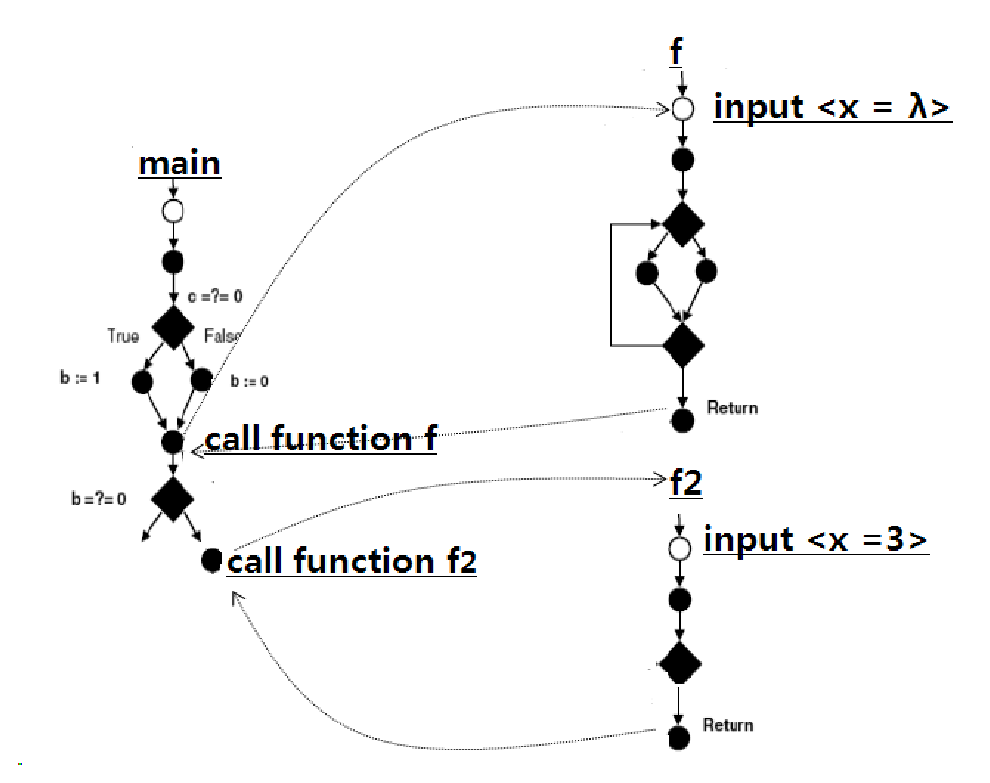
\includegraphics[scale=0.6,clip]{fig/selective.eps} 
\caption{\label{fig:s2e}Example of selective symbolic execution} 
\end{figure}


Selective symbolic execution (S$^2$E) has two dimensions in a system; code and data. Users can specify portions of code of interest by indicating file name or range of program counters. Given code information, S$^2$E executes the portion of code symbolically. All variables in the portion in conditional branches are involved in symbolic execution. Therefore, all paths could be explored symbolically. Users can specify portions of data of interest by indicating a data structure's name or address range of data segment. Then, S$^2$E executes all portion of code related to the data of interest symbolically.
Figure~\ref{fig:s2e} shows an example of S$^2$E execution. In the example, the main function calls functions $f$ and $f_2$. Consider that users specify $f$ is portion (of interest) to be executed symbolically. To achieve the goal, when the main function calls the $f$ that has an input parameter $X$, $X$ is assigned to a symbolic value, $\lambda$ and $f$ is symbolically executed. However, when the main function calls the $f_2$ of non-interest, S$^2$E assigns $X$ as ``3'' to execute $f_2$ concretely.


